\chapter[Referencial Teórico]{Referencial Teórico}\label{chap:refteor}
Este Capítulo apresenta as bases teóricas que apóiam esse trabalho. Organizado em seções, têm-se:
Seção de \hyperref[sec:sisrec]{Sistemas de Recomendação}, que apresenta o 
conceito de Sistemas de Recomendação; Seção de \hyperref[sec:ia]{Inteligência Artificial}, a qual traz 
o conceito e recursos desta que serão utilizados neste trabalho; Seção \hyperref[sec:expus]{Experiência do usuário},
que aborda a experiência do usuário e sua importância para este trabalho. Por fim, na Seção 
\hyperref[sec:resrefteor]{Resumo do Capítulo} são apresentadas as considerações finais
do capítulo.

\section{Sistemas de Recomendação}\label{sec:sisrec}

Os Sistemas de Recomendação são aplicações de software que analisam e processam dados dos usuários com o propósito de 
sugerir itens que possam ser de interesse desses usuários. Assim, eles ajudam os usuários a descobrir novos produtos, 
conteúdos ou serviços que possam ser do seu interesse, personalizando suas experiências \cite{pham2019recommendation}.

\begin{figure}[htbp]
    \centering
    \caption{Ciclo dos Sistemas Recomendação}
    \label{fig:ciclosr}
    
    \vspace{2pt} % Espaço vertical entre a legenda e a imagem
    
    \includegraphics[width=0.5\textwidth]{figuras/ciclosr.eps}
    
    \vspace{2pt} % Espaço vertical entre a imagem e a fonte da imagem
    
    \small Fonte: Autora
\end{figure}

O processo utilizado em um sistema de recomendação pode ser dividido em várias etapas, como demonstrado na Figura 
\hyperref[fig:ciclosr]{1}. O ciclo começa na coleta de dados (Coletar). Nesta etapa, o sistema coleta dados relevantes para análise
do perfil do usuário, tais como: interações com o sistema; \textit{feedbacks}, e fontes externas como sociais. Todos esses são dados válidos. 
Como \mycitetext{10.1145/2959100.2959120} exemplificam, o Spotify coleta informações dos artistas, sinais acústicos das músicas, histórico, 
além de músicas ouvidas em tempo real.
Após a coleta, ocorrem o armazenamento e a filtragem desses dados (Armazenar e Filtrar). Em geral, o intuito é popular a 
base de dados. Quanto maior a quantidade de dados,
melhor para a análise. Há necessidade ainda de separar esses esses dados para melhorar a acurácia do modelo \cite{pham2019recommendation}.
Em seguida, 
tem-se a análise desses dados (Analisar). No caso desse trabalho, serão utilizados algoritmos de \textit{deep learning} para detectar padrões,
e encontrar as preferências do usuário. Dessa forma, será possível gerar recomendações em potencial (Gerar), 
as quais serão sugeridas para o usuário, entrando na última parte do ciclo, que é a avaliação pelo usuário da 
recomendação (Avaliar). Com base nessa avaliação, o modelo de recomendação 
recebe mais dados do perfil daquele usuário e o ciclo recomeça, retornando à etapa de coleta de dados (Coletar).

\section{Inteligência Artificial}\label{sec:ia}

Inteligência Artificial é um conjunto de tecnologias que permitem aos computadores executar uma variedade de 
funções avançadas, incluindo a capacidade de ver, entender e traduzir idiomas falados e escritos; analisar dados; 
fazer recomendações, e muito mais \cite{Suleimenov}.

No contexto de Sistemas de Recomendação, é feito o uso principalmente de cinco técnicas da Inteligência Artificial 
\cite{stratoflow-recommendation}:
\begin{itemize}
\item Filtros colaborativos: essa técnica foca na similaridade entre diferentes usuários e itens. Usuários que são
similares, provavelmente, possuem o mesmo tipo de interesse \cite{pham2019recommendation}, como demonstrado na Figura 
\hyperref[fig:filtrocolab]{2};

\begin{figure}[htbp]
    \centering
    \caption{Filtro Colaborativo}
    \label{fig:filtrocolab}
    
    \vspace{2pt} % Espaço vertical entre a legenda e a imagem
    
    \includegraphics[width=0.5\textwidth]{figuras/filtrocolab.eps}
    
    \vspace{2pt} % Espaço vertical entre a imagem e a fonte da imagem
    
    \small Fonte: Autora
\end{figure}

\item Filtros de conteúdo: essa técnica avalia a similaridade entre os itens. Itens similares aos que o usuário gostou/visualizou
possuem mais probabilidade de serem de seu interesse \cite{stratoflow-recommendation}, 
como demonstrado na Figura 
\hyperref[fig:filtrocont]{3};

\begin{figure}[htbp]
    \centering
    \caption{Filtro de Conteúdo}
    \label{fig:filtrocont}
    
    \vspace{2pt} % Espaço vertical entre a legenda e a imagem
    
    \includegraphics[width=0.5\textwidth]{figuras/filtrocontent.eps}
    
    \vspace{2pt} % Espaço vertical entre a imagem e a fonte da imagem
    
    \small Fonte: Autora
\end{figure}

\item Filtros demográficos: essa técnica busca categorizar os usuários com base em atributos, fazendo recomendações
com base em características demográficas específicas dos usuários \cite{burke2002hybrid}. Por exemplo, no comércio eletrônico, 
essa técnica pode separar os clientes por gênero, segmentando os produtos com base em categorias 
tradicionalmente associadas ao gênero, tais como uma seção de roupas femininas e outra seção de roupas masculinas. Ou ainda,
pode separar os clientes por localização, fornecendo roupas mais frescas para cliente cuja localização está em áreas mais quentes,
e roupas mais agasalhadas para cliente cuja localização está em áreas mais frias;

\item Filtros baseados em conhecimento e utilidade: essa técnica recomenda com base nas necessidades dos usuários, 
calculando a utilidade de cada item para o usuário. Para isso, é necessário conhecimento do que o usuário precisa e 
quais os itens que suprem essa necessidade \cite{burke2002hybrid}. Por exemplo, um usuário pesquisa por um restaurante
italiano específico (como Peccorino). Então o sistema de recomendação buscaria quais são os itens que tem maior utilidade para 
o usuário, nesse caso, sugerindo outro restaurante italiano similar;

\item Filtros Híbridos: essa técnica combina outras técnicas de filtragem, como por exemplo Filtros colaborativos e Filtros
de conteúdo. Possui várias formas de combinar essas técnicas, que serão abordadas na seção 
\hyperref[subsubsec:tiposfh]{Classificação de Filtros Híbridos}. Esta técnica consegue lidar com as limitações das técnicas que 
ela combina. Pode-se, por exemplo, lidar com usuários de gostos diferenciados, além de situações nas quais se
têm poucos dados de interação do usuário. Portanto, isso confere uma forma de tratar o problema de 
"partida a frio" \cite{stratoflow-recommendation}, e 

\item Filtros baseados em \textit{Deep Learning}: essa técnica utiliza das outras técnicas de filtragem e 
aplica sistemas redes neurais para fazer predições e recomendações, 
como Redes Neurais Convolucionais (RNC), para dados mais voltados para imagens, e Redes Neurais Recorrentes (RNR), para dados
sequênciais \cite{nvidia-recommendation}.
\end{itemize}

Para esse trabalho, serão abordados de forma mais aprofundada os seguintes filtros:
\hyperref[subsec:hibridos]{Filtros Híbridos} e \hyperref[subsec:filtrodeep]{Filtros baseados em \textit{Deep Learning}}.

\subsection{Filtros Híbridos}\label{subsec:hibridos}
A filtragem híbrida aborda mais de um tipo de técnica de filtragem, visando mitigar aspectos negativos que essas filtragens
possuem ao serem tratadas separadamente, tais como os problemas de \textit{cold start}; diversidade, e esparcidade dos dados. 
Esse modelo, também surgiu
na tentativa de melhorar a acurácia do processo de recomendação \cite{thorat2015survey}.

\subsubsection{Classificação de Filtros Híbridos}\label{subsubsec:tiposfh}
De acordo com \mycitetext{burke2002hybrid}, os modelos com filtragem híbrida voltados para Sistemas de Recomendação podem possuir
várias classificações com base em como combinam os tipos de filtro. Alguns dessas classificações são:

\begin{itemize}
    \item Por peso (\textit{Weighted}): Apresenta um sistema de peso, onde o peso de um item é calculado com base no resultado
    de sua avaliação por todas as técnicas presentes no sistema. Esse tipo toma como base o fato de que todas as técnicas 
    produzem valores relativos similares. Entretanto, isso nem sempre é o caso. Assim, alguns itens com poucas classificações 
    podem ser ignorados;

    \item Por troca (\textit{Switching}): Ocorre troca entre diferentes técnicas de recomendação dependendo do contexto.
    Esse tipo adiciona uma complexidade a mais ao sistema, já que precisa definir o critério para troca entre as técnicas,
    mas também permite aproveitar os benefícios de várias técnicas;

    \item Por mistura (\textit{Mixed}): Apresenta recomendações de mais de uma técnica juntas. Esse modo reduz parcialmente
    o problema de "patida à frio". Para novos itens é possível classificá-los com base em suas descrições. Porém, para novos 
    usuários, o problema de não ter informações suficiente permanece; 

    \item Por combinação de \textit{features} (\textit{Feature Combination}): Usa os dados do filtro colaborativo como dados
    adicionais associados a exemplo. Adicionalmente, usa filtros de conteúdos na base aumentada que será gerada. Esse tipo considera
    os dados gerados pelos filtros colaborativos, sem necessariamente depender deles. Assim reduz o problema da falta de dados
    \textit{cold start};

    \item Por cascata (\textit{Cascade}): Usa uma técnica para produzir uma classificação grosseira dos dados. Em seguida, 
    usa outra técnica para refinar essa classificação. Esse tipo evita que itens sejam ignorados, como pode ocorrer na técnica
    de peso, na qual aplica a técnica a todos os itens. No tipo cascata, as classificações são apenas refinadas e não substituidas; 

    \item Por aumento de \textit{features} (\textit{Feature Augmentation}): Usa um modelo gerado por uma técnica de filtro
    para produzir uma classificação ou avaliação de um item. Essa informação produzida vai ser introduzida em outro 
    modelo, gerado por outra técnica de filtro, a ser utilizada na sequência. Esse tipo de
    sistema hibrído pode aumentar o desempenho do sistema sem modificá-lo diretamente, e

    \item Por \textit{Meta-level} (\textit{Meta-level}): Usa um dos modelos gerados pelas técnicas como entrada 
    para o outro modelo, sendo esse último gerado por outra técnica.
    Por exemplo, usar o modelo gerado por filtros colaborativos como entrada para um modelo gerado por filtro de conteúdo.
    Nesse caso em específico, o \textit{Meta-level} tem o benefício de que o modelo final vai ser uma representação fiel
    dos interesses do usuário, facilitando a operação do sistema ao usar essa representação na comparação com dados crus 
    de avaliação.
\end{itemize}

O Quadro \hyperref[tab:1]{1} mostra exemplos de sistemas existentes, possíveis ou propostos com as possíveis combinações de 
filtros hibrídos. Nas linhas temos as possíveis combinações entre filtros, por exemplo, FC/FPC que seria Filtro Colaborativo 
em conjunto com Filtro Por Conteúdo. Nas colunas temos as classificações dos diferentes tipos de filtros hibrídos, por exemplo,
por combinação de \textit{features}. Nesse sentido, temos exemplos citados pelo autor de modelos que existem ou foram propostos
para cada combinação entre os filtros em cada uma das classificações. Existindo casos que ou não é possível a implementação
dessa combinação de filtros com a classificação especifica, por exemplo a combinação de Filtro Colaborativo com Filtro demográfico
na aplicação por \textit{Meta-level}. Ou ainda que é redudante o uso da combinação de filtros com a classificação, como no exemplo
da combinação de Filtro Por Conteúdo com Filtro Colaborativo em quatro casos (por peso, por mistura, por troca e 
por combinação de \textit{features}), pois para esses casos é indiferente a ordem dos filtros então se usamos primeiro Filtro Por Conteúdo
ou Filtro Colaborativo o resultado seria o mesmo, por isso redundante.

\begin{table}[htbp]
    \centering
    \small % Reduzindo o tamanho da fonte
    \begin{threeparttable}
        \caption{Modelos possíveis, existentes (ou propostos) de recomendação híbrida}
        \label{tab:1}
        \begin{tabular}{|>{\centering\arraybackslash}m{1.67cm} *{7}{>{\centering\arraybackslash}m{1.8cm}}|}
        \hline  
        & Por peso & Por mistura & Por troca & Por combinação de \textit{features} & Por cascata & Por aumento de \textit{features} & Por \textit{Meta-level} \\
        \hline 
        FC/FPC & P-Tango & PTV, ProfBuilder & DailyLearner & (Basu, Hirsh, \& Cohen 1998) & Fab & Libra &  \\
        \hline  
        FC/FD & (Pazzani 1999) &  &  &  &  &  & Não é possível \\
        \hline  
        FC/FBCU & (Towle \& Quinn 2000) &  & (Tran \& Cohen, 2000) & Não é possível &  &  &  \\
        \hline  
        FPC/FC & Redundante & Redundante & Redundante & Redundante &  &  & Fab, (Condliff, et al. 1999), LaboUr \\
        \hline  
        FPC/FD & (Pazzani 1999) &  &  & (Condliff, et al. 1999) &  &  & Não é possível \\
        \hline  
        FPC/FBCU &  &  &  & Não é possível &  &  & \\
        \hline  
        FD/FC & Redundante & Redundante & Redundante & Redundante &  &  & Não é possível \\
        \hline  
        FD/FPC & Redundante & Redundante & Redundante & Redundante &  &  &  \\
        \hline  
        FD/FBCU &  &  &  & Não é possível &  &  &  \\
        \hline  
        FBCU/FC & Redundante & Redundante & Redundante & Redundante & EntreeC & GroupLens (1999) &  \\
        \hline  
        FBCU/FPC & Redundante & Redundante & Redundante & Redundante &  &  &  \\
        \hline  
        FBCU/FD & Redundante & Redundante & Redundante & Redundante &  &  & Não é possível \\
        \hline  
        \end{tabular}
        \begin{tablenotes}
            \small
            \centering
            \item Fonte: \cite{burke2002hybrid} - Tradução (Autora)
            \item Legenda: (FC = Filtro Colaborativo, FPC = Filtro Por Conteúdo, 
            FBCU = Filtro Baseado em conhecimento e utilidade, FD = Filtro demográfico)
        \end{tablenotes}
    \end{threeparttable}
\end{table}

\subsubsection{Possíveis implementações}\label{subsubsec:implemfh}
No contexto desse trabalho, o filtro híbrido a ser discutido será uma combinação de filtros colaborativos e filtros de 
conteúdo. No quesito de implementação da combinação desses filtros, fortemente baseada nas classificações dos filtros 
híbridos, encontram-se as possibilidades exemplificadas por 
\mycitetext{thorat2015survey}:

\begin{itemize}
    \item Implementar os filtros separadamente, combinando-os depois para realizar a recomendação, como exemplificado na Figura
    \hyperref[fig:combind]{4};

    \begin{figure}[H]
        \centering
        \caption{Combinação individual}
        \label{fig:combind}
        
        \vspace{2pt} % Espaço vertical entre a legenda e a imagem
        
        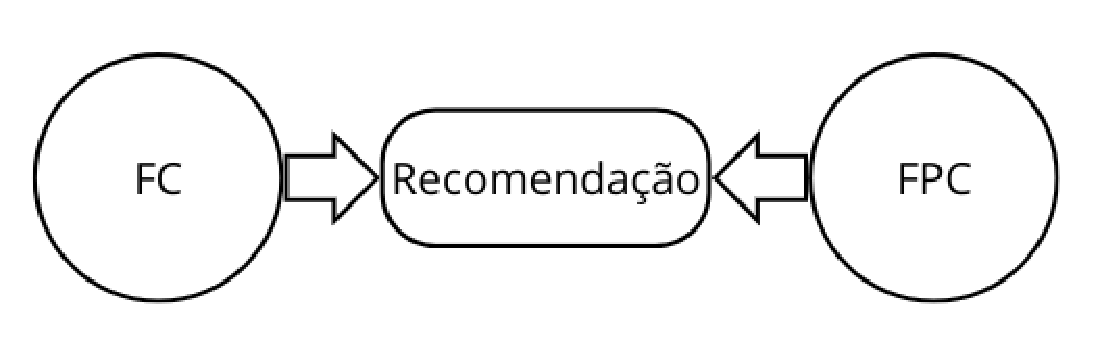
\includegraphics[width=0.5\textwidth]{figuras/combin2.eps}
        
        \vspace{2pt} % Espaço vertical entre a imagem e a fonte da imagem
        
        \small Fonte: \cite{thorat2015survey} - Tradução (Autora)
    \end{figure}

    \item Implementar características do filtro de conteúdo no filtro colaborativo, como exemplificado na Figura
    \hyperref[fig:cfcbf]{5};

    \begin{figure}[H]
        \centering
        \caption{Agregar conteúdo dentro de colaborativo}
        \label{fig:cfcbf}
        
        \vspace{2pt} % Espaço vertical entre a legenda e a imagem
        
        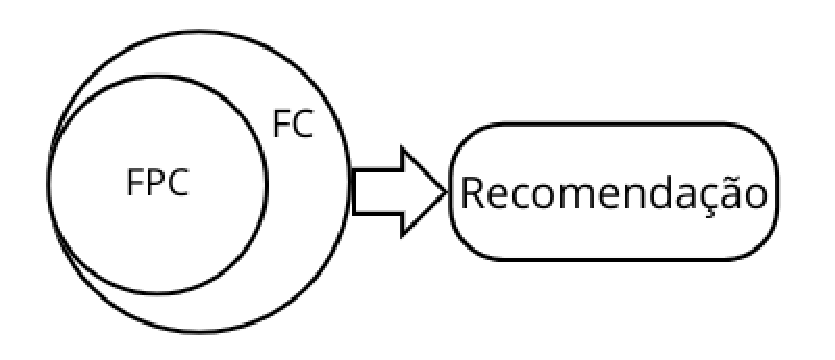
\includegraphics[width=0.5\textwidth]{figuras/cfcbf2.eps}
        
        \vspace{2pt} % Espaço vertical entre a imagem e a fonte da imagem
        
        \small Fonte: \cite{thorat2015survey} - Tradução (Autora)
    \end{figure}

    \item Unificar os filtros em um único modelo, como exemplificado na Figura
    \hyperref[fig:modelounico]{6}, e

    \begin{figure}[H]
        \centering
        \caption{Ambos os filtros em um único modelo}
        \label{fig:modelounico}
        
        \vspace{2pt} % Espaço vertical entre a legenda e a imagem
        
        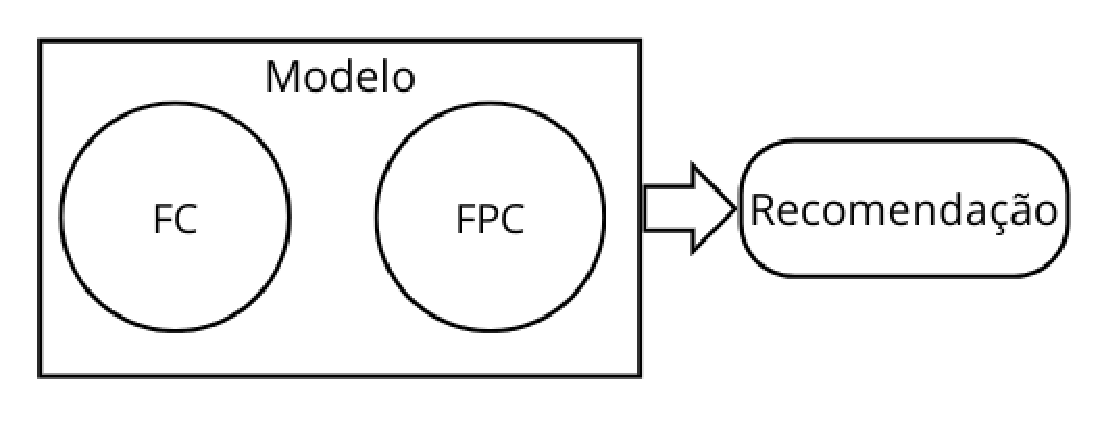
\includegraphics[width=0.5\textwidth]{figuras/modelounico2.eps}
        
        \vspace{2pt} % Espaço vertical entre a imagem e a fonte da imagem
        
        \small Fonte: \cite{thorat2015survey} - Tradução (Autora)
    \end{figure}

    \item Implementar características do filtro colaborativo no filtro de conteúdo, como exemplificado na Figura
    \hyperref[fig:cbfcf]{7}.

    \begin{figure}[H]
        \centering
        \caption{Agregar colaborativo dentro de conteúdo}
        \label{fig:cbfcf}
        
        \vspace{2pt} % Espaço vertical entre a legenda e a imagem
        
        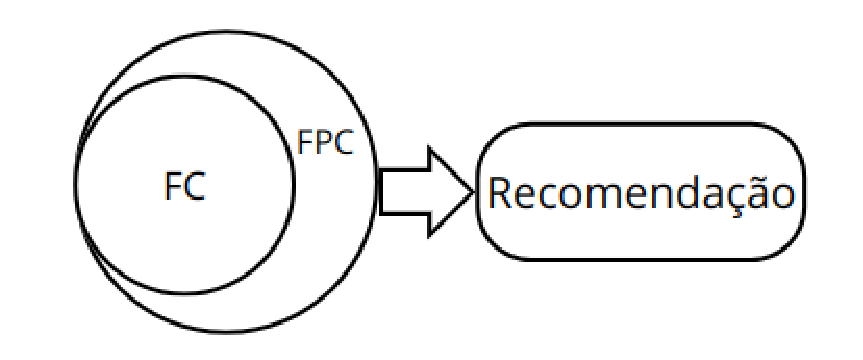
\includegraphics[width=0.5\textwidth]{figuras/cbfcf2.eps}
        
        \vspace{2pt} % Espaço vertical entre a imagem e a fonte da imagem
        
        \small Fonte: \cite{thorat2015survey} - Tradução (Autora)
    \end{figure}
\end{itemize}

\subsection{Filtros Baseados em \textit{Deep Learning}}\label{subsec:filtrodeep}
\textit{Deep Learning} é uma sub-área de Inteligência Artificial que se concentra no treinamento de algoritmos para 
realização de tarefas complexas de forma autônoma. Permite ainda que esses algoritmos aprendam representações de 
dados com múltiplas camadas de abstração \cite{LeCun2015}. Focando em Sistemas de Recomendação, 
pode-se melhorar outros filtros existentes ao usar \textit{Deep Learning}. Nesse sentido, há quatro possíveis 
abordagens: Redes Neurais Convolucionais; Redes Neurais Recorrentes; Máquina de Boltzmann Restrita e Autoencoder 
\cite{elSisi2020}.

\subsubsection{Redes Neurais Convolucionais}\label{subsubsec:rnc}
É um tipo de rede neural com camadas convolucionais e operações de agrupamento \cite{elSisi2020}.

No escopo de Sistemas de Recomendação, são ideais para processar dados de multimídia, conseguindo associar dados de 
diferentes formatos, melhorando a precisão das recomendações.

\subsubsection{Redes Neurais Recorrentes}\label{subsubsec:rnr}
É um tipo de rede neural que possui \textit{loops} e guarda cálculos anteriores. Ideal para modelar dados sequenciais 
\cite{elSisi2020}.

Aplicando esse método em Sistemas de Recomendação, consegue-se identificar padrões no comportamento e nas interações dos usuários,
e criar recomendações baseadas na navegação do usuário na rede, sem precisar de dados iniciais informados pelos
usuários. Esse último caso ocorre na geração de \textit{cookies} \cite{elSisi2020}. Dessa forma, pode-se lidar com o problema 
da "partida a frio".

\subsubsection{Máquina de Boltzmann Restrita}\label{subsubsec:boltzmann}
A Máquina de Boltzmann Restrita é uma rede neural de dupla camada, sendo uma visível e outra escondida \cite{elSisi2020}. 

Para Sistemas de Recomendação, pode ser interligada com filtros colaborativos, aumentando o tamanho da base de dados, e
melhorando o processo de recomendação \cite{elSisi2020}. Ela também pode ser treinada para aprender uma representação
dos padrões de interação entre usuários e itens para, posteriormente, gerar recomendações com base nas preferências dos
usuários e nas características dos itens.

\subsubsection{\textit{Autoencoder}}\label{subsubsec:autoencoder}
\textit{Autoencoder} é uma rede neural que tenta reconstruir seu dado de entrada em um dado similar na saída, ao usar uma
camada mediadora \cite{elSisi2020}. Sendo assim, possui três camadas, nas quais o número de neurônios na entrada deve ser igual ao número de
neurônios na saída, como exemplificado na Figura \hyperref[fig:autoencoder]{8}.

\begin{figure}[H]
    \centering
    \caption{Estrutura de um \textit{Autoencoder}}
    \label{fig:autoencoder}
    
    \vspace{2pt} % Espaço vertical entre a legenda e a imagem
    
    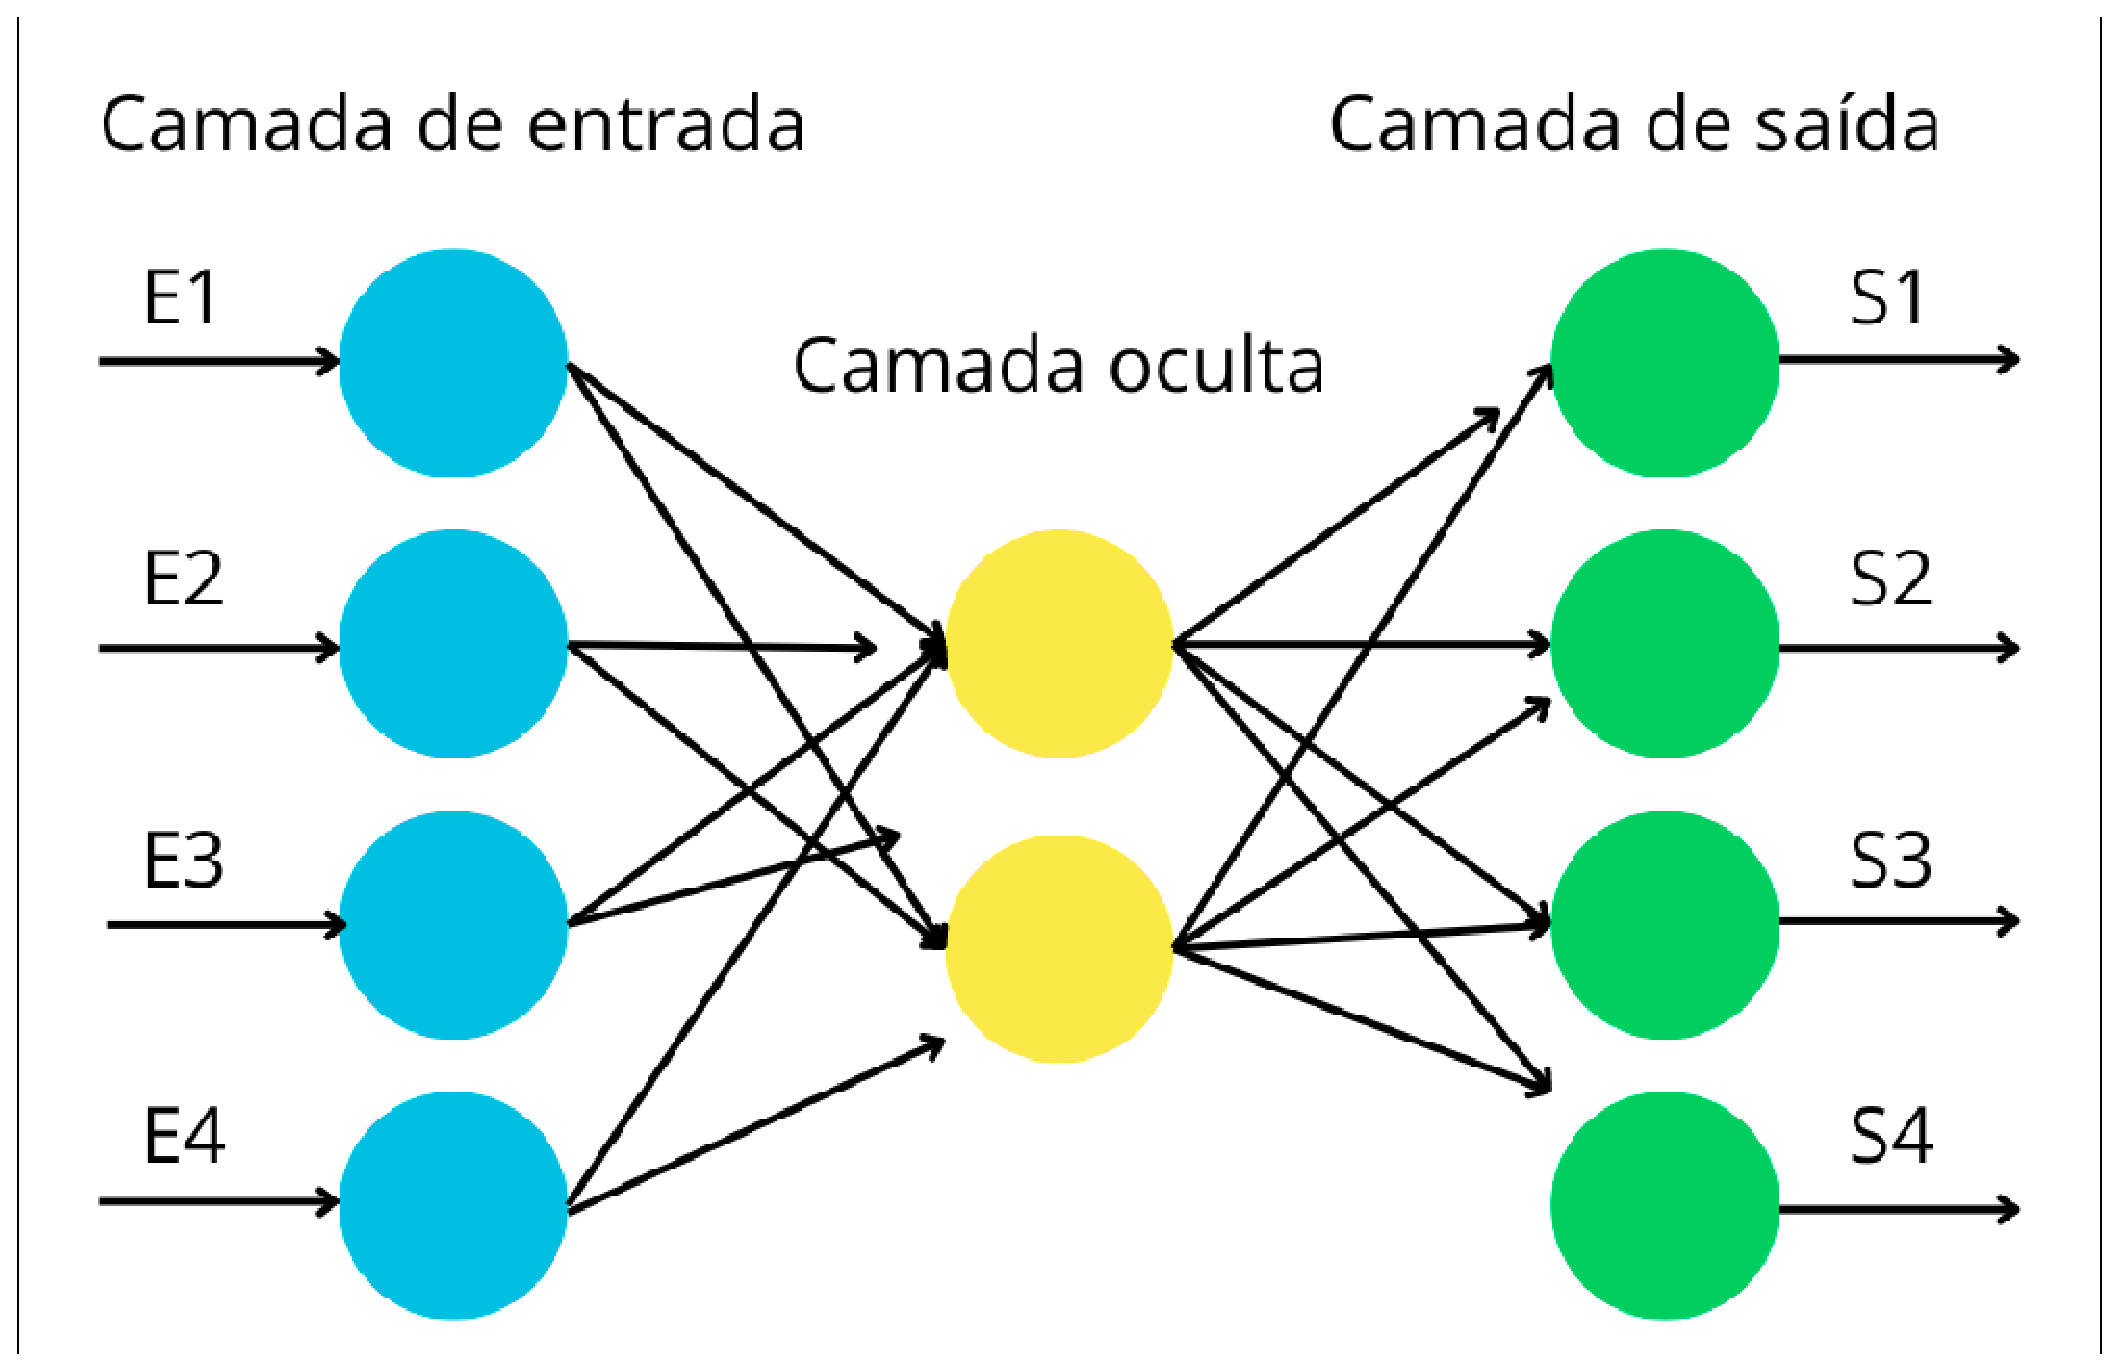
\includegraphics[width=0.5\textwidth]{figuras/autoencoder2.eps}
    
    \vspace{2pt} % Espaço vertical entre a imagem e a fonte da imagem
    
    \small Fonte: \cite{elSisi2020} - Tradução (Autora)
\end{figure}

No contexto de Sistemas de Recomendação, essa rede neural tem a habilidade de reduzir e reconstruir os dados, extraindo os 
atributos destes. Por isso, um \textit{Autoencoder} pode ser treinado para aprender representações latentes dos itens, as 
quais capturam as características
essenciais dos itens e podem ser usadas para recomendar itens semelhantes com base em similaridade. Essa rede neural pode ser 
usada para aprender representações dos usuários e itens a partir de interações históricas de usuários com itens, provendo
recomendações com base em padrões de comportamento. Por fim, pode-se ainda aprender diferentes tipos de informações com
base em diferentes tipos de dados de entrada (ex. áudio, imagem e texto), combinando essas modalidades para gerar a recomendação \cite{zhang2020autoencoder}.

% \subsection{Modelo a ser usado}\label{subsec:modeloaserusado}

\section{Satisfação do Usuário}\label{sec:expus}
A satisfação de um usuário durante o uso de um sistema é subjetiva, e vária de acordo com os elementos característicos do
sistema, os gostos e percepções do usuário, bem como a tarefa que estão realizando naquele sistema \cite{griffiths2007user}.
Ainda de acordo com \mycitetext{griffiths2007user}, a satisfação do usário tem o objetivo de de prover à um sistema pontos 
relevantes sobre sua performance e da própria experiência do usuário ao usar o sistema. 

No quesito de experiência do usuário, esta pode ser definida como as respostas e percepções de uma pessoa ao usar um produto, 
sistema ou serviço \cite{iso9241-210}. Entretanto, também é possível dizer que a experiência de usuário vai além de avaliar a 
usabilidade/funcionalidade durante
a interação do usuário. Na verdade, a experiência de usuário tende a cobrir não só os comportamentos do sistema, bem como a 
eficiência e a efetividade \cite{allam2013user}. 

\mycitetext{applegate1993models} mostra que existem três modelos de satisfação do usuário: modelo de satisfação material, modelo de satisfação emocional simples e 
modelo de satisfação emocional múltiplo. Porém esses modelos são subjetivos e difíceis de mesurar. 
Assim, de acordo com \mycitetext{zviran2003measuring} vários estudiosos desenvolveram diferentes ferramentas para tentar mesurar 
a satisfação
do usuário, como Bailey e Pearson que criaram um questionário de 39 itens com diferentes métodos de construção. Porém, 
\mycitetext{zviran2003measuring} ainda trás que apesar de todos os estudos a cerca do tema, nem sempre as resposatas são
precisas. Dessa forma, os estudos sobre o tema continuaram e novos modelos foram desenvolvidos.

No contexto desse trabalho, será considerado o modelo de \mycitetext{mahmood2000variables} que tem três focos principais:
\begin{itemize}
    \item Benefícios e conveniência: voltado para expectativa do usuário, facilidade de uso e utilidade percebida;
    \item Antecedentes do usuário: voltado para a experiência do usuário ao utilizar o sistema, 
    habilidades do usuário com sistemas similares e envolvimento do 
    usuário no desenvolvimento do sistema, e
    \item Suporte e estímulo organizacional: voltado para a atitude do usuário em relação ao sistema de informação, o qual
    avalia o grau de satisfação com o sistema de informação provido pela organização,    
    e suporte organizacional, o qual indica grau de apoio da organização para facilitar o uso e a adoção do sistema.
\end{itemize}
Para o ponto de suporte/estímulo organizacional, será considerado da autora como a organização provedora do sistema.

Dessa forma, esse trabalho tem o intuito de levantar considerações dos usuários acerca do sistema, e usar esses
dados para avaliar um Sistema de Recomendação centrado em Inteligência Artificial. Para isso, será desenvolvido e treinado um
modelo se Sistema de Recomendação, o qual será integrado em uma API (se traduz para Interface de Programação de Aplicações), que
será disponibilizada para testes com um conjunto de usuários.E em seguida, será apresentado um questionário para os usuários,
baseados nos focos do modelo de \mycitetext{mahmood2000variables}, para determinar a satisfação deles com o sistema. E, com base 
nas respostas será incrementado a base de dados do modelo dados extraídos dos questionários e treinado novamente o modelo, 
sendo apresentado mais uma vez aos usuários gerando uma segunda onda de respostas às quais serão comparadas com
a primeira e analisado se houve evolução do sistema.

\section{Resumo do Capítulo}\label{sec:resrefteor}

Esse capítulo apresentou uma ideia geral do que são Sistemas de Recomendação. Trata-se de um sistema que visa recomendar coisas que 
sejam do interesse dos usuários, usuários. Esse processo envolve etapas, sendo as mesmas: Coletar Dados, 
Armazenar Dados, Filtrar Dados, Analisar Dados, Gerar Recomendações e Avaliar Recomendações. 
Foram abordados diversos filtros para Sistemas de Recomendação usando Inteligência 
Articial, sendo eles: colaborativo, por conteúdo, demográfico, baseado em conhecimento e utilidade, híbridos e baseados em
\textit{Deep Learning}.

Com foco em filtros híbridos e filtros baseados em \textit{Deep Learning}, foi detalhado mais como eles funcionam e suas definições.
Para os filtros híbridos, que são combinações de outros filtros (colaborativo e por conteúdo, no contexto deste trabalho),
foi apresentada sua classificação: por peso, que pondera os resultados dos filtros que são combinados; por mistura, que 
apresenta em conjunto os resultados dos outros filtros; por troca, que alterna entre os filtros com base em um critério;
por combinação de \textit{features}, que usa dados de um dos filtros para aumentar a base de dados do outro filtro a ser usado;
por cascata, que usa um filtro para produzir uma classificação e outro filtro para refinar essa classificação; por aumento
de \textit{features}, que o resultado de um filtro é a entrada de outro filtro; e por último por \textit{Meta-level}, que
o modelo gerado por um filtro é usado de entrada em outro filtro.

Para os filtros baseados em \textit{Deep Learning}, foram cobertos quatro metódos, sendo eles: Redes Neurais 
Convolucionais, que auxiliam na interpretação e na associação de diferentes formatos de dados; Redes Neurais Recorrentes, 
que aprendem padrões de uso do usuário; Máquina de Boltzmann Restrita, que geram representações de usuários
e itens para melhorar o processo de recomendação; e por fim Autoencoder, que pode tanto combinar diferentes multimídias, quanto 
gerar representações de usuários para melhorar as recomendações.

Essa capítulo ainda trata a satisfação do usuário em Sistemas de Recomendação, e como isso será abordado
no trabalho.